\documentclass[../main.tex]{subfiles}

\begin{document}
The thesis focuses on implementing a safe learning controller for an inverted pendulum. Initially, a Markov Decision Process model of the pendulum system is obtained by essentially discretizing the state and action space, assigning rewards to the discrete states and calculating transition probabilities between the single states. As in \cite{akametalu2014reachability}, a system with an unknown state-dependent disturbance $d(x)$ that is added to the known part of the system dynamics is assumed. Additionally, a conservative initial disturbance bound $\overline{d}_0$ and $\underline{d}_0$ is assumed to be known initially that will be iteratively updated with a Gaussian Process model. Based on the initial disturbance estimate and a safe set, the backwards reachable set that should be avoided in order to never leave the safe set is calculated with HJI reachability analysis. This calculation gives rise to a safe region within the state space within which the learning controller can operate freely. Additionally, the safe set calculations output a safe controller that should be applied at the borders of this set. Based on that, the chosen Reinforcement Learning algorithm can learn a policy by choosing actions and receiving subsequently information about the reward and the state transition associated with that action. If the chosen action would yield the system to leave the safe region, the safe controller acts and brings the system back into the safe set. The chosen Reinforcement Learning algorithm is a modified version of Delayed Q-Learning introduced in section \ref{sec:RL}.

While the learning controller acts, data samples are recorded and subsequently fed into the Gaussian Process model. The Gaussian Process estimates a less conservative bound for the disturbance so that subsequently a larger safe set can be calculated with HJI reachability analysis. This procedure is sketched in figure \ref{fig:flow_simple}. The estimated safe set is fed into the safe learning controller that learns a policy through interaction with the system. The during the learning recorded samples are used to get a better estimate of the disturbance that results in a less restrictive safe control.\par
\begin{figure}
    \centering
    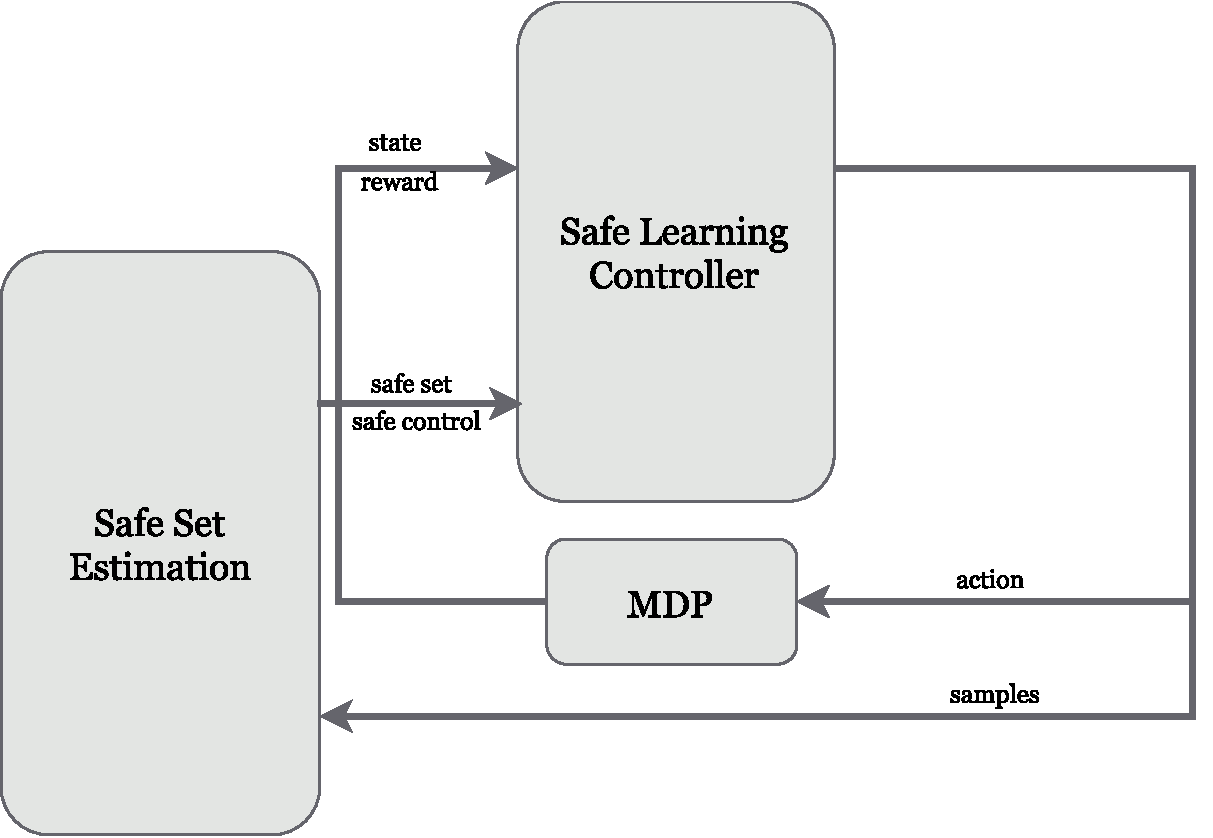
\includegraphics[width=\textwidth]{flow_simple}
    \caption{Rough Control Setup.}
    \label{fig:flow_simple}
\end{figure}
In more detail, the same control scheme is explained in figure \ref{fig:flow_complete}. In this figure the colours blue and red are used to underline the two control loops that run in parallel: The blue loop is the safety loop, that estimates the disturbance, calculates a safe set and a safe controller on that basis and checks every action that the learning controller wants to take. The red loop is the learning control loop where the Reinforcement Learning controller chooses an action based on its policy, and subsequently receives some feedback from the process. Based on the received reward the controller updates its policy. For each action that the learning controller chooses, the safe controller performs a check if that action would violate the boundaries of the safe set. If that is the case, the action is not executed but replaced by a safety-preserving action.
\begin{figure}
    \centering
    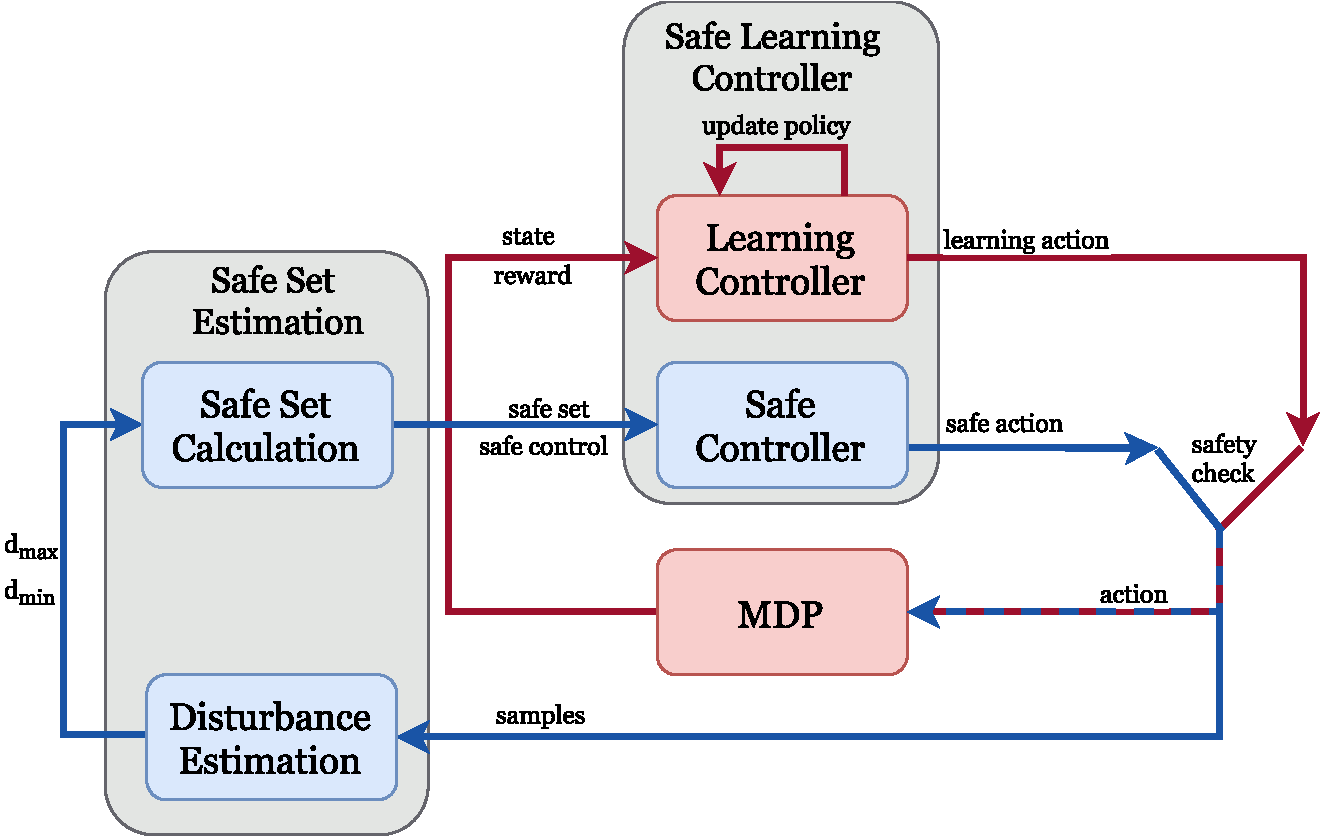
\includegraphics[width=\textwidth]{flow_complete}
    \caption{Detailed Control Setup.}
    \label{fig:flow_complete}
\end{figure}
This very rough sketch will be further explained in section \ref{sec:Implementation}.

\end{document}